%---------------------------------------------------------
%	TITLE SLIDE
%---------------------------------------------------------
\section{}

% Set background
\usebackgroundtemplate{%
    \begin{tikzpicture}
        \clip (0,0) rectangle (\paperwidth,\paperheight); % crop the 3:2 photo to 16:9 without stretching
        \node[inner sep=0, opacity=0.25] at ({0.5\paperwidth},{0.5\paperheight}) {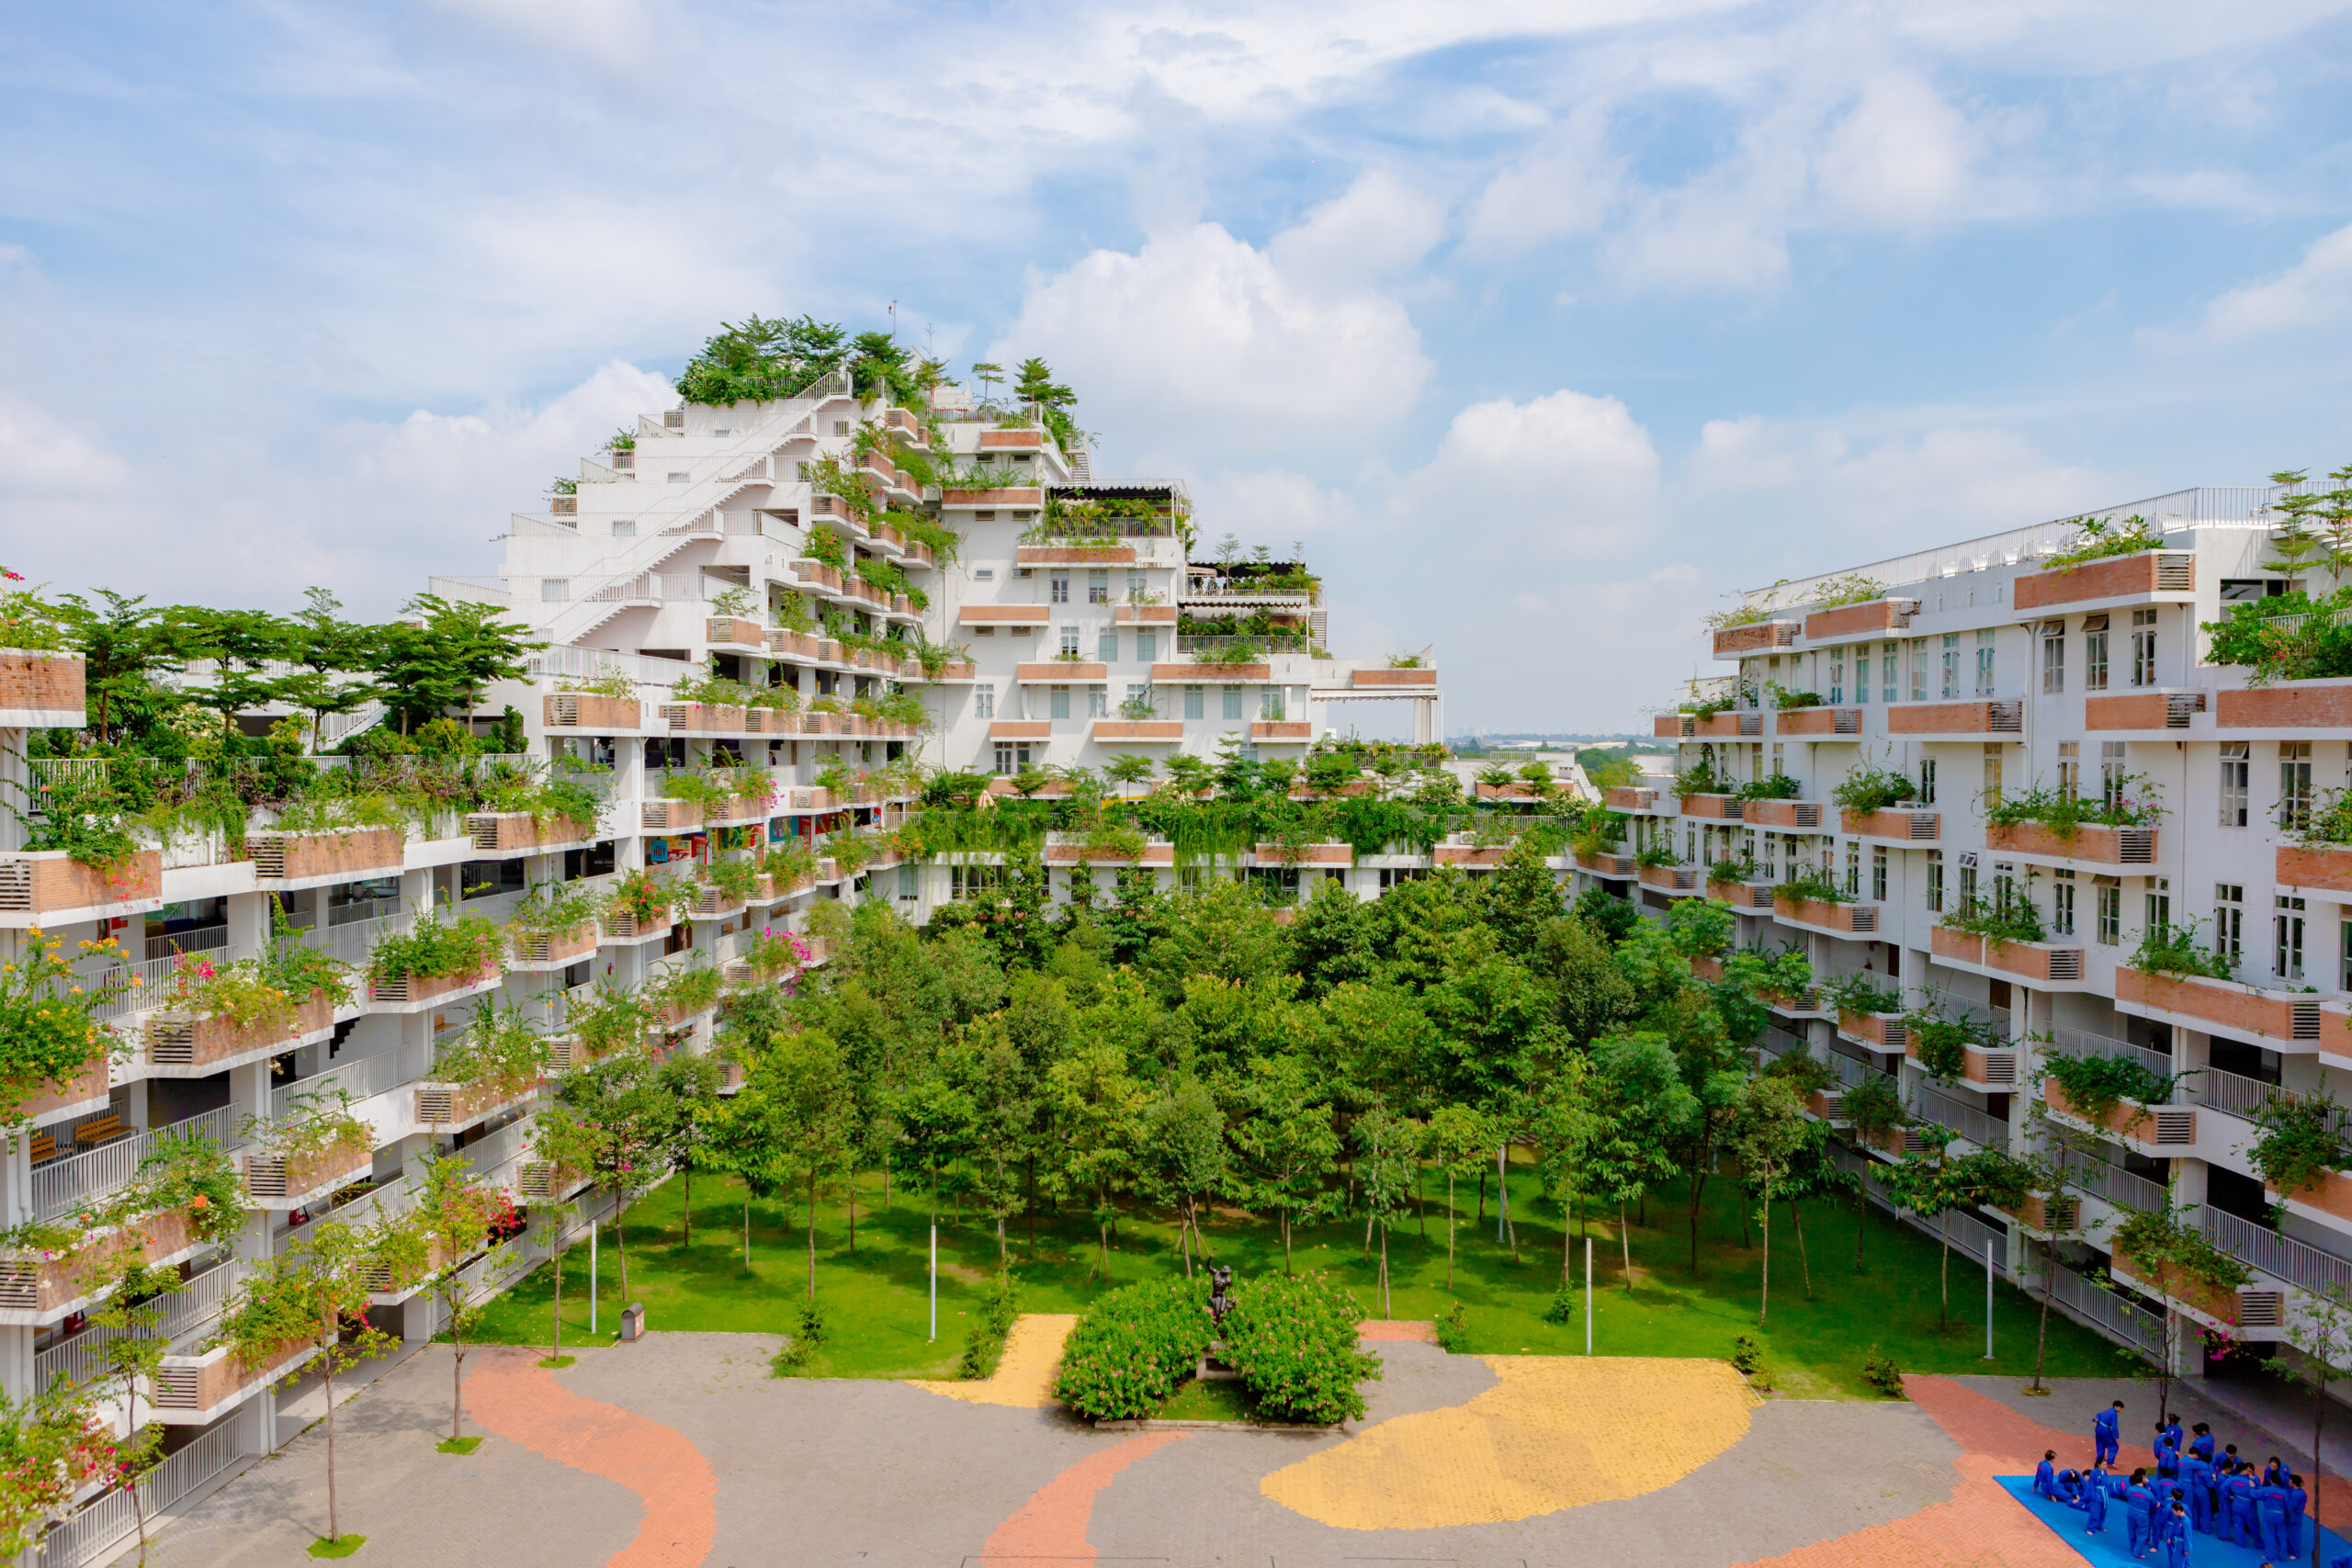
\includegraphics[width=\paperwidth]{P.Zo-9862-scaled-1.jpg}};
        % FPT logo top-left, just below the headline and above the title box
        \node[anchor=north west, inner sep=0] at (4mm,{\paperheight-0.9cm}) {
\includegraphics[height=0.85cm]{Logo_FPT_Education.png}};
    \end{tikzpicture}%
}
% Disable logo
\logo{}

\begin{frame}
	\titlepage % Output the title slide, automatically created using the text entered in the PRESENTATION INFORMATION block above
\end{frame}

% Clear background
\usebackgroundtemplate{}
% Enable logo
\logo{\fptlogo}

% Switch to Theme III
\setbeamercolor{section in head/foot}{fg=fptOrange, bg=white}
\setbeamercolor{title in head/foot}{fg=white, bg=fptOrange}
\setbeamercolor{headline}{fg=fptOrange, bg=white}
